%!Tex Program = xelatex
\documentclass{beamer}

\usepackage{ctex}
\usepackage{graphicx}
\usepackage{subfigure}
%\usetheme[]{Antibes}
\usepackage{cite}
% Removes icon in bibliography
\setbeamertemplate{bibliography item}[text]


\title{Equipotential Lines}
\author{物200 曾剑涛 20003157}
\date{}

\begin{document}
    \maketitle

    %\tableofcontents

    \section{题目和翻译}
    \begin{frame}
        \frametitle{题目和翻译}

        Place two electrodes into water, supply a safe voltage and use a voltmeter to 
        determine electric potential at various locations. Investigate how the measured
         equipotential lines deviate from your expectations for different conditions
          and liquids.

        将两个电极放入水中,加一个安全的电压,然后使用电压表测定不同位置的并绘制等势线。研究测
        出的等势线与期望条件下的偏差。研究不同的条件和液体种类对误差的影响。
    \end{frame}

    \section{实验原理}
    \begin{frame}
        \frametitle{实验原理}
        可以用恒定电流唱模拟静电场进行静电场的测绘。常用平等输电线模拟点电荷的电场,用同轴电缆
        模拟同轴圆柱带电体的电场。
        
        用恒定电流场模拟静电场的条件:

        恒定电流场的导电物质应是不良导体,导电率远低于金属电极。

        实验室中通常使用石墨导电纸纸作为导电介质。
        
        是否可以用水作为导电介质进行静电场的测绘?
    
    \end{frame}

    \begin{frame}
        \frametitle{同轴电缆模拟同轴圆柱带电体}
        \begin{figure}
            \centering
            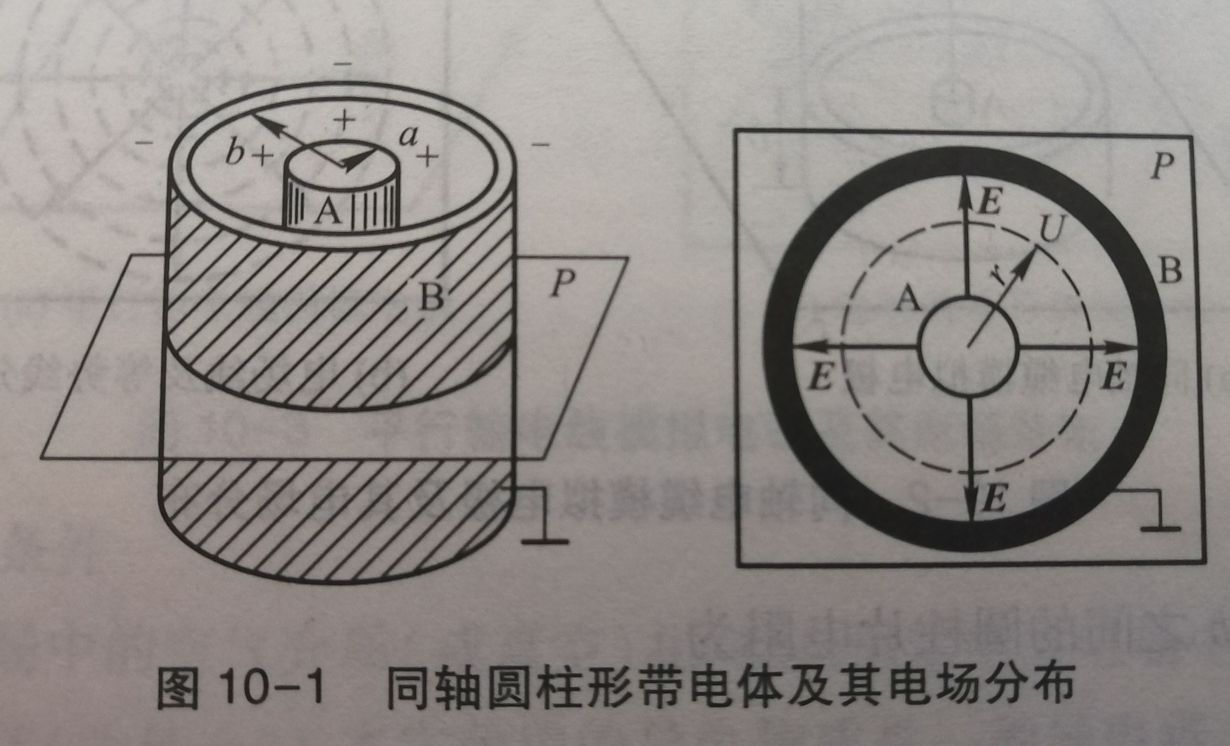
\includegraphics[width=7cm]{同轴圆柱带电体}
            \caption{同轴圆柱形带电体及其电场分布}
        \end{figure}
        其电势分布为$$ U_r = U_a \frac{\ln \frac{b}{r}}{ \ln \frac{b}{a}{} } $$
        
    
    \end{frame}

    \begin{frame}
        \frametitle{同轴电缆模拟同轴圆柱带电体}
        \begin{figure}
            \centering
            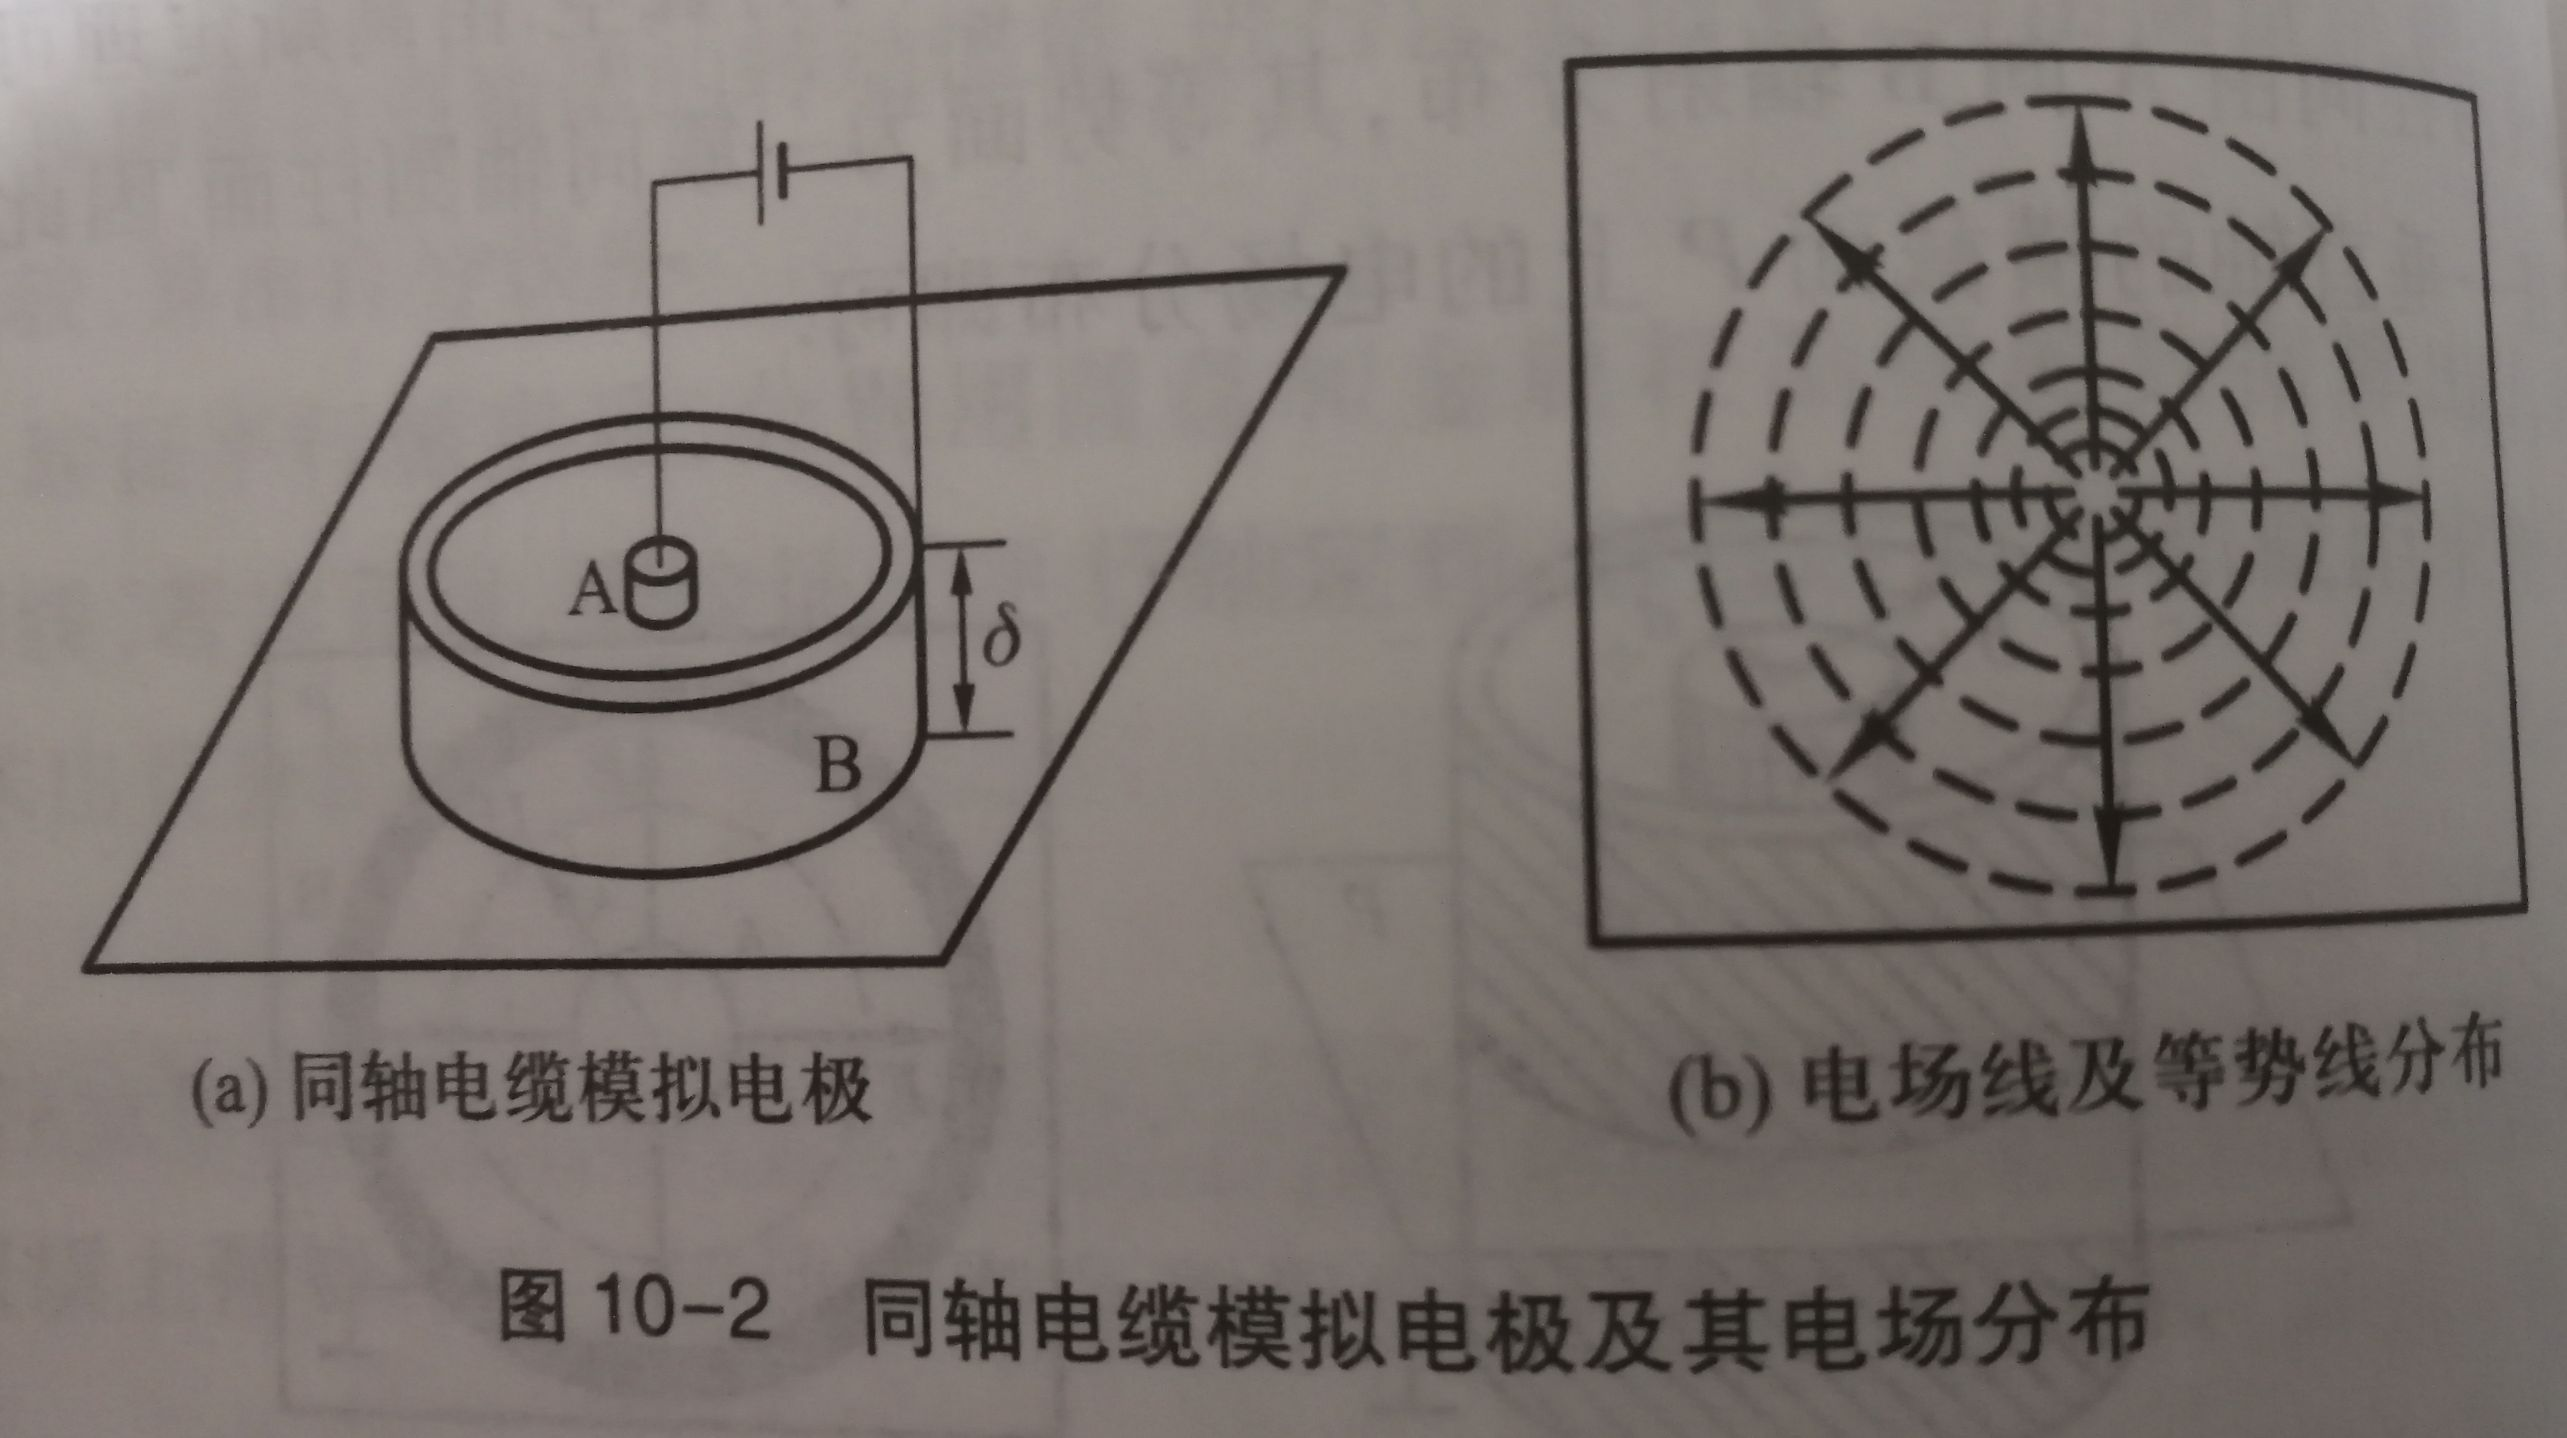
\includegraphics[width=7cm]{同轴电缆}
            \caption{同轴圆电缆模拟电极及其电场分布}
        \end{figure}
        其电势分布为$$ U_r = U_a \frac{\ln \frac{b}{r}}{ \ln \frac{b}{a}{} } $$
        
    
    \end{frame}

    \begin{frame}
        \frametitle{导电介质对测绘的影响}
        
        \begin{columns}
            \begin{column}{.5\linewidth}
                
        $$ R_{ar} = \int_{a}^{r} \frac{\rho}{2 \pi h} \times \frac{dr}{r} = \frac{\rho}{2 \pi h} \ln \frac{r}{a}$$
        $$ R_{rb} = \int_{r}^{b} \frac{\rho}{2 \pi h} \times \frac{dr}{r} = \frac{\rho}{2 \pi h} \ln \frac{b}{r}$$
        $$ R_{rb} = \int_{a}^{b} \frac{\rho}{2 \pi h} \times \frac{dr}{r} = \frac{\rho}{2 \pi h} \ln \frac{b}{a}$$
        未接探测电路(电压表)时,$$U_r = \frac{U_a}{R_{ab}} \times R_{rb} = U_a \frac{\ln \frac{b}{r}}{\ln \frac ba}$$
        
        \end{column}
            \begin{column}{.5\linewidth}
                \begin{figure}[h]
                    \centering
                    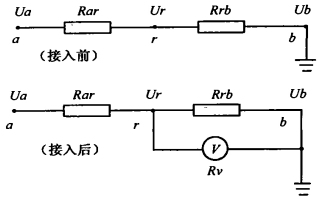
\includegraphics[width=4.5cm]{接入探测电路前后的等效电路}
                    \caption{接人探测线路前后的等效电路}
                \end{figure}
            \end{column}

        \end{columns}

        
    \end{frame}

    \begin{frame}
        \frametitle{导电介质对测绘的影响}
        
           
        接入电压表后,$$U_r' = \frac{U_a}{R_{ar} + R_{rb} // R_v} \times ({R_{ar} + R_{rb} // R_v}) 
        = U_a[\frac{\ln \frac{b}{r}}{\ln \frac ba + \frac{1}{R_v} \cdot \frac{\rho}{2 \pi h} \ln \frac ra \ln \frac br  }] $$
        
        $$
        \Delta U = |U_r - U_r'| = U_a[ \frac{\ln \frac br}{\ln \frac ba} -  \frac{\ln \frac{b}{r}}{\ln \frac ba + 
            \frac{1}{R_v} \cdot \frac{\rho}{2 \pi h}
             \ln \frac ra \ln \frac br  } ]
        $$
        
        由此可见, 在接入电压表时,电压表的内阻$R_v$和导电介质的性能
        会对测量结果造成影响。电压表内阻$R_v$越大,导电介质(水)电阻率$\rho$越小,水深$h$
        越大,测量结果越精确。

        

    \end{frame}
    
    \section{实验内容}

    \begin{frame}
        \frametitle{实验装置}
        \begin{figure}
            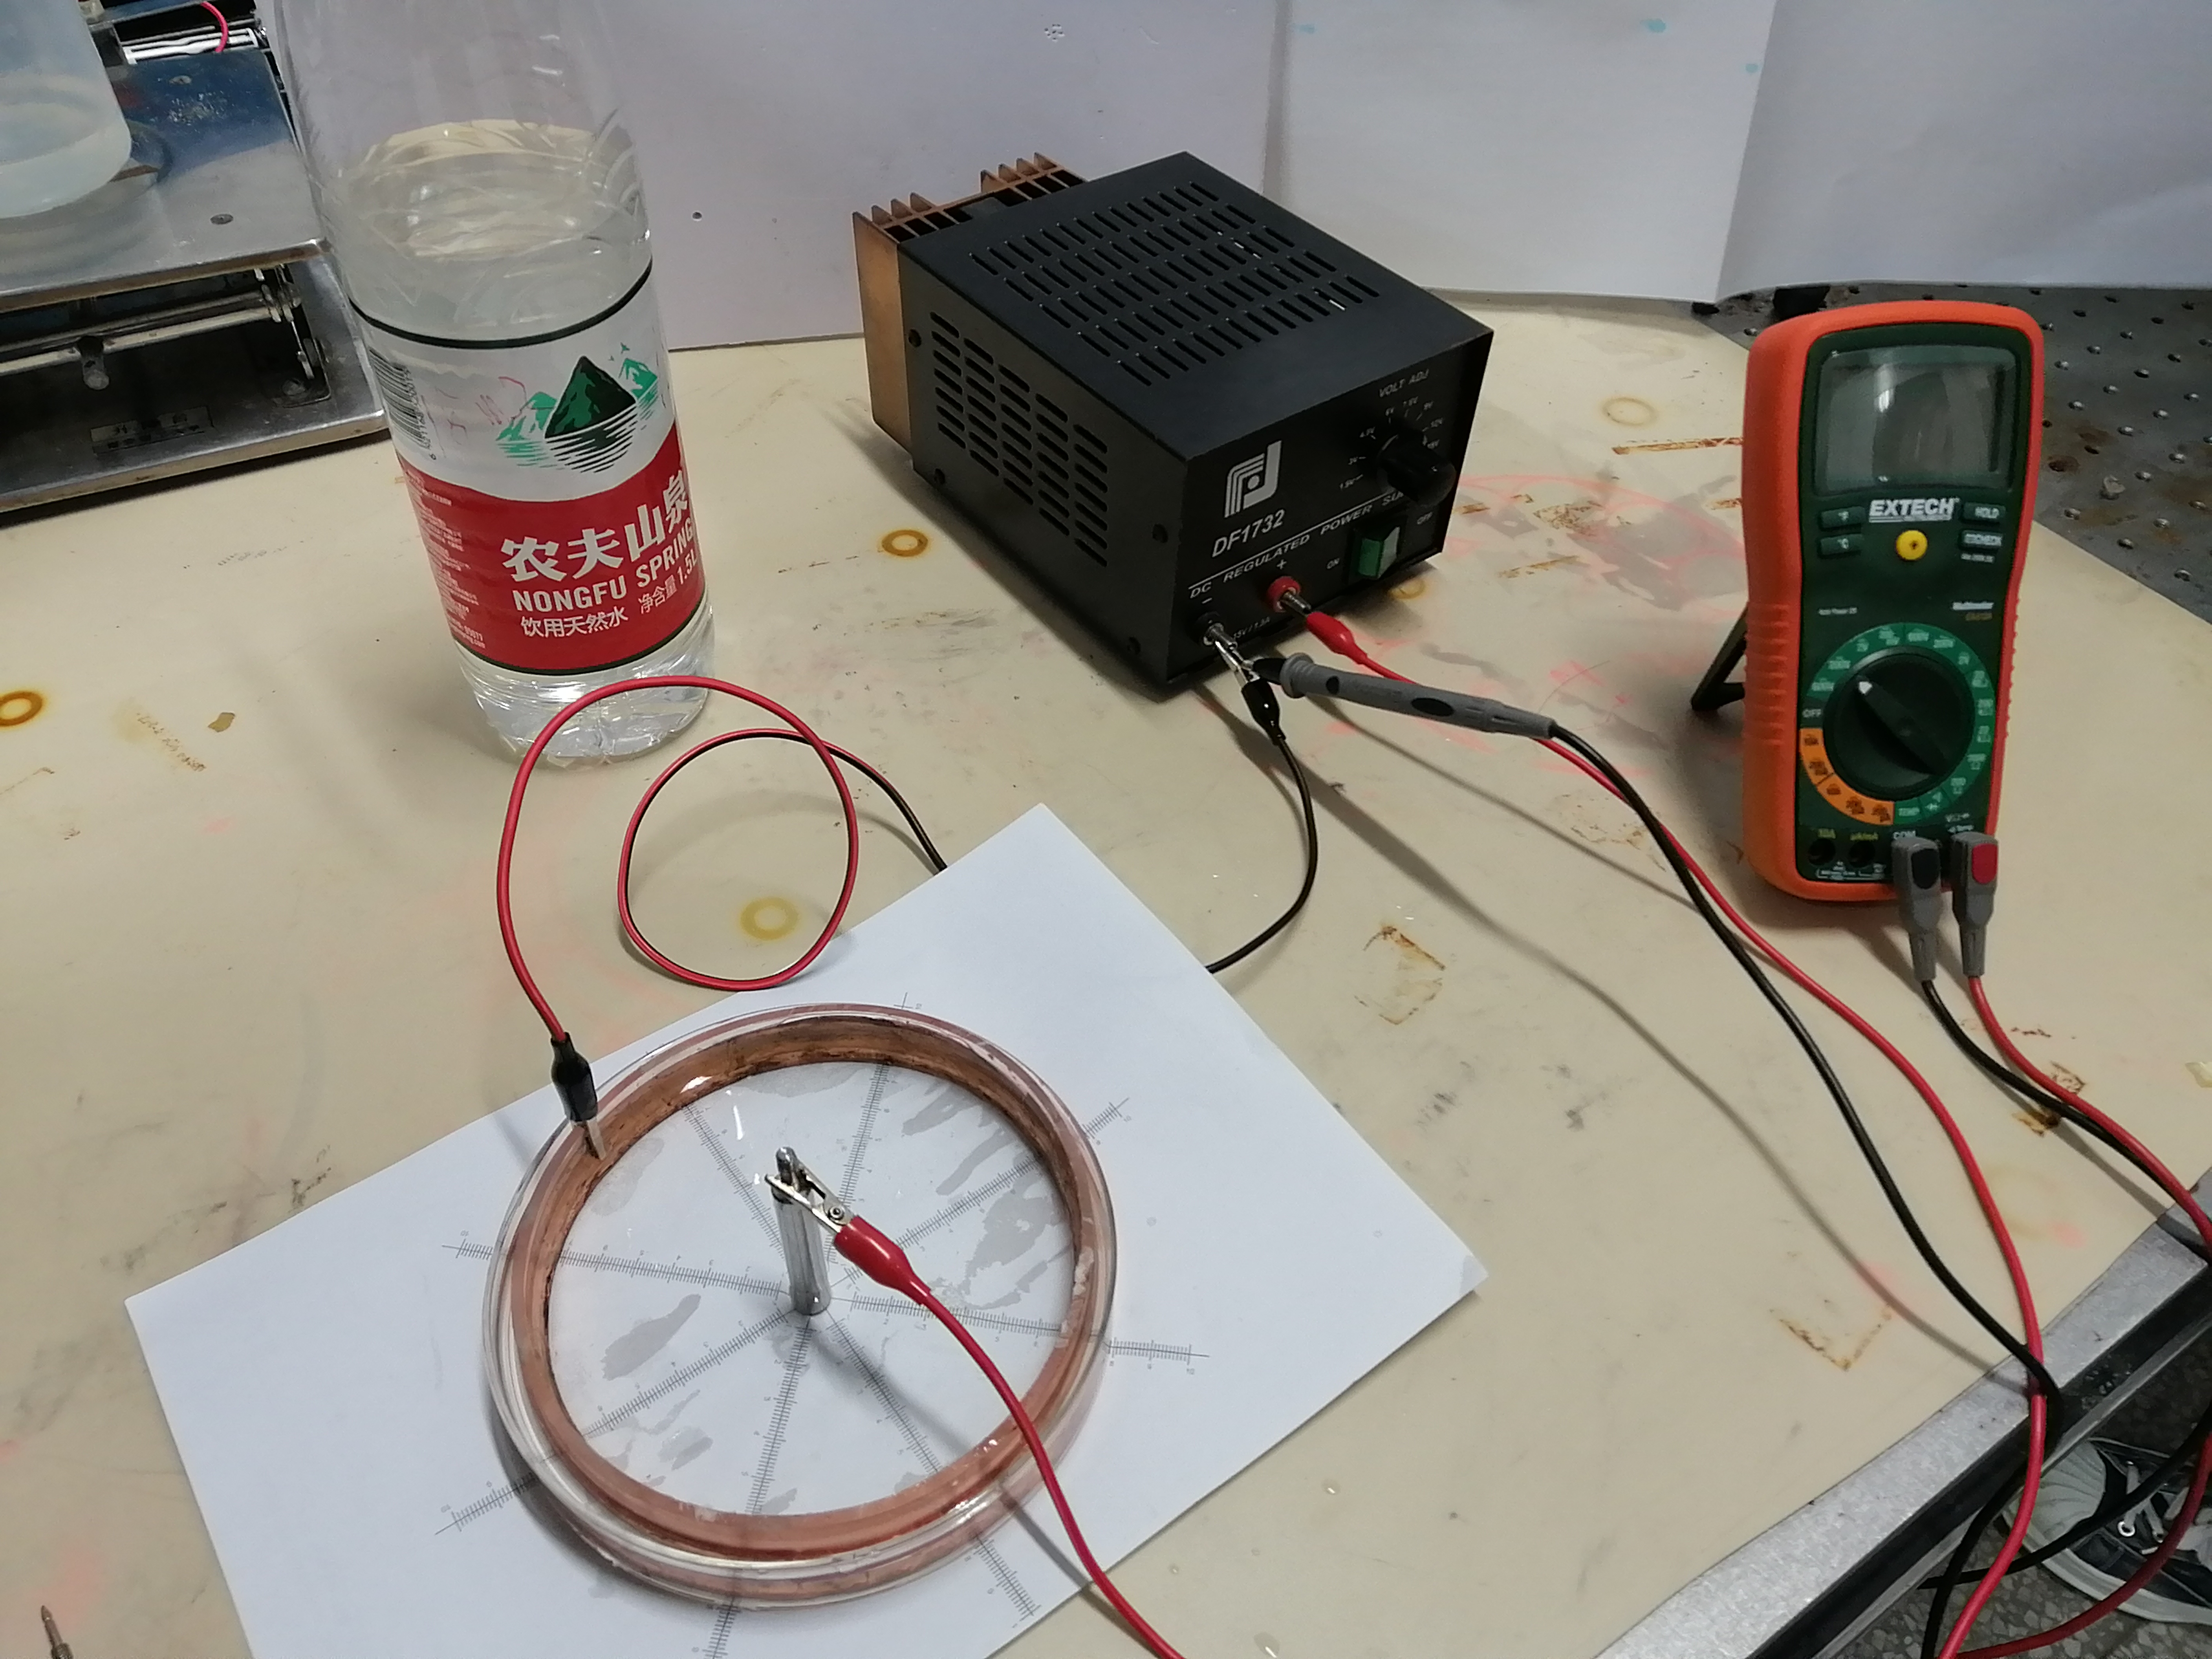
\includegraphics[width=6.5cm]{实验装置}
            \caption{实验装置}
        \end{figure}
        我们利用以上实验装置,控究了液体种类(电阻率)和水深对测量结果的影响。
    \end{frame}

    \begin{frame}
        \frametitle{实验数据}
        水深的影响:
        \begin{figure}
            \subfigure[]{
                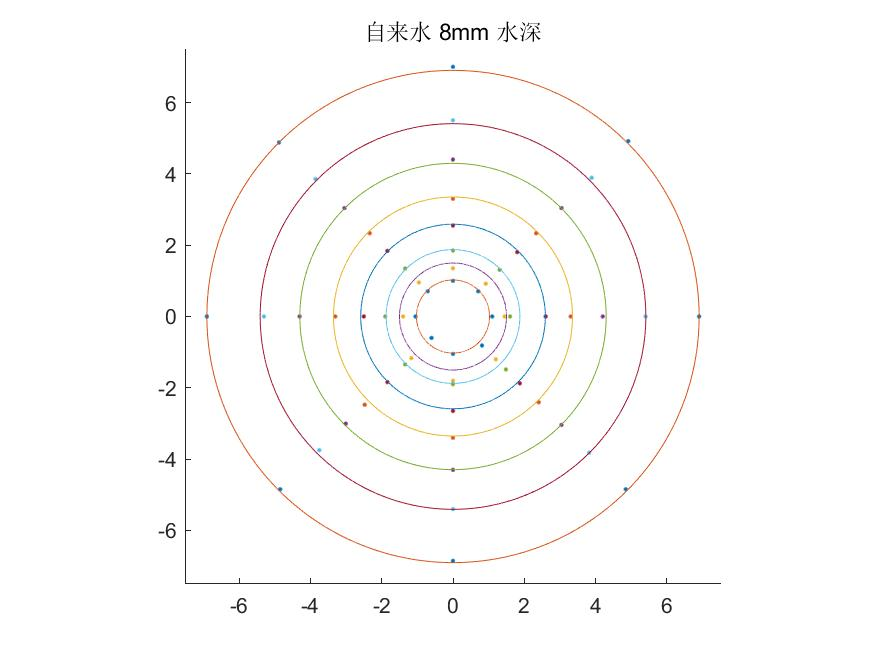
\includegraphics[width=.3\linewidth]{1.jpg}
            }
            \subfigure[]{
                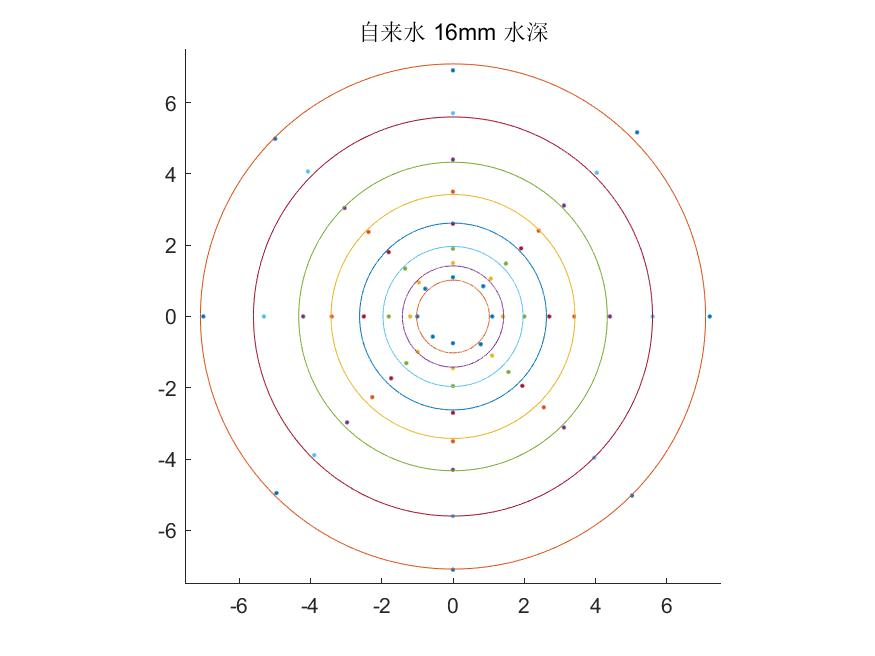
\includegraphics[width=.3\linewidth]{2.jpg}
            }
            \subfigure[]{
                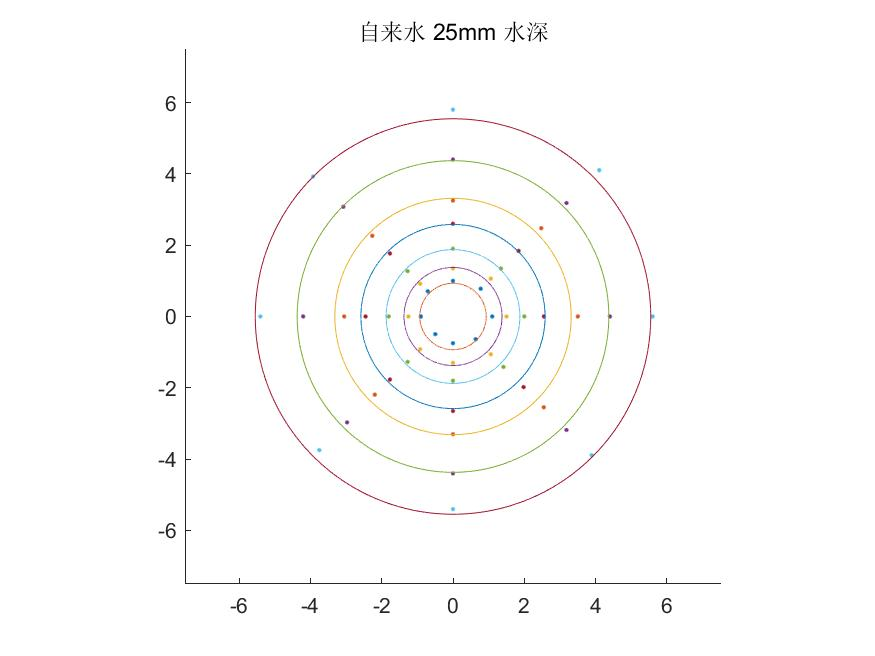
\includegraphics[width=.3\linewidth]{3.jpg}
            }
            \caption{自来水在8mm,16mm,25mm三种水深时的测绘结果。}

        \end{figure}
        \begin{table}[width=\linewidth]
            %\setlength{\tabcolsep}{1mm}{
            \begin{tabular}{|c|c|c|c|c|c|c|c|c|}
            \hline
            U/V  & 8    & 7    & 6    & 5    & 4    & 3    & 2    & 1    \\ \hline
            R/cm & 1.03 & 1.50 & 1.88 & 2.59 & 3.35 & 4.29 & 5.41 & 6.90 \\ \hline
            R/cm & 1.02 & 1.42 & 1.96 & 2.62 & 3.42 & 4.33 & 5.59 & 7.08 \\ \hline
            R/cm & 0.93 & 1.38 & 1.88 & 2.58 & 3.31 & 4.37 & 5.54 & NaN  \\ \hline
            \end{tabular}
            %}
        \end{table}

    \end{frame}

    \begin{frame}
        \frametitle{实验数据}
        水深的影响:
        \begin{figure}
            \subfigure[]{
                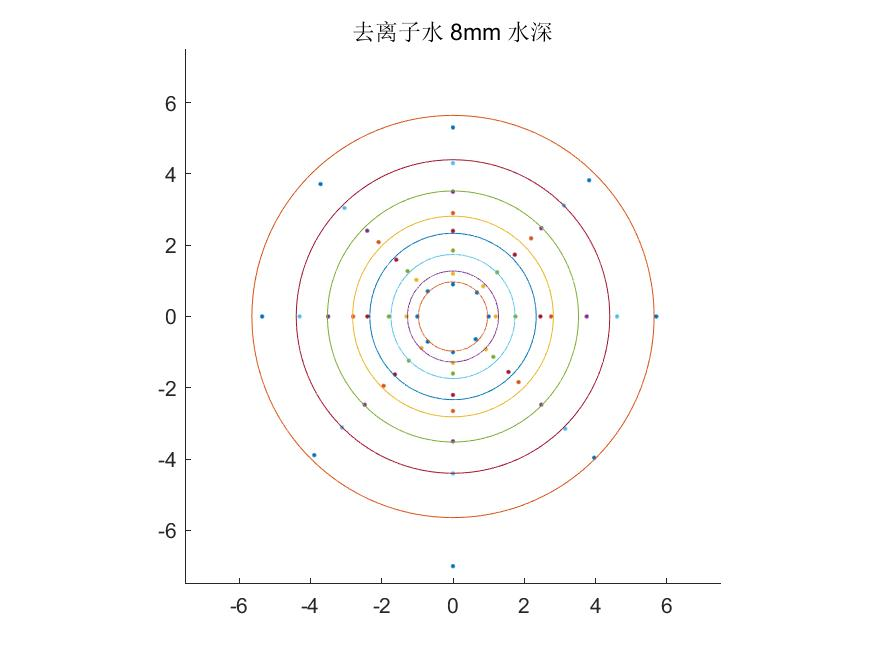
\includegraphics[width=.3\linewidth]{4.jpg}
            }
            \subfigure[]{
                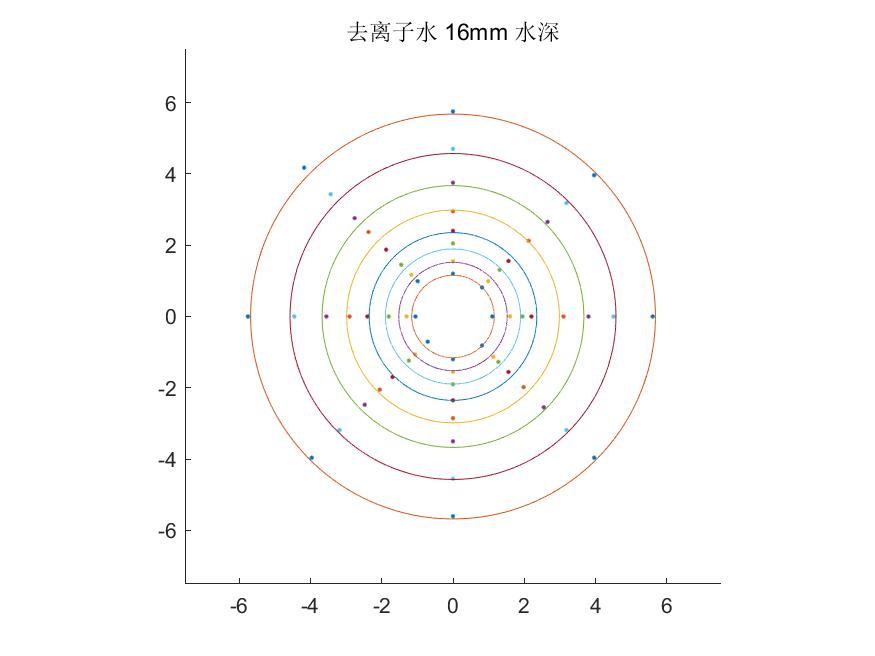
\includegraphics[width=.3\linewidth]{5.jpg}
            }
            \subfigure[]{
                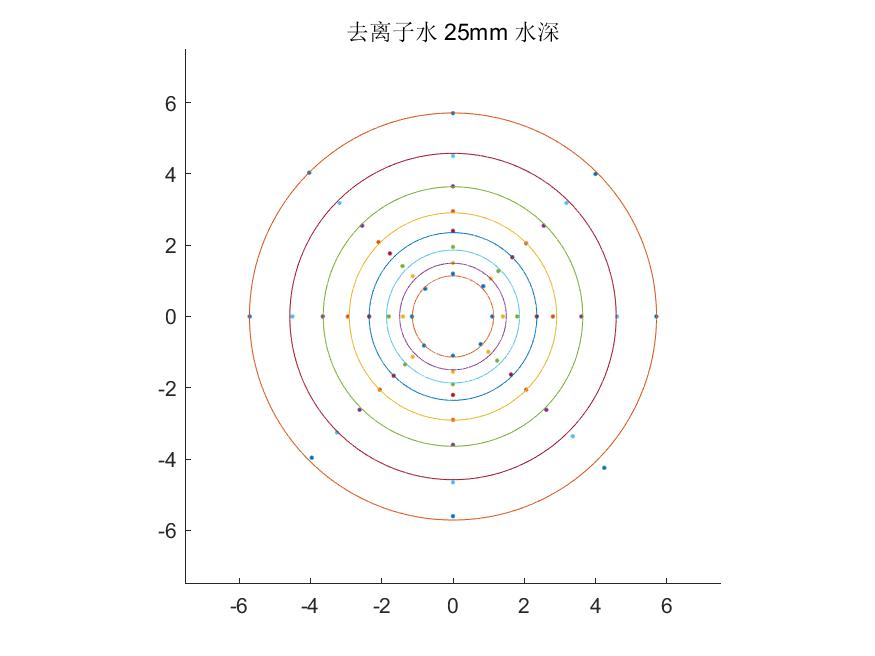
\includegraphics[width=.3\linewidth]{6.jpg}
            }
            \caption{去离子水在8mm,16mm,25mm三种水深时的测绘结果。}

        \end{figure}

        \begin{table}[width=\linewidth]
            %\setlength{\tabcolsep}{1mm}{
            \begin{tabular}{|c|c|c|c|c|c|c|c|c|}
            \hline
            U/V  & 8    & 7    & 6    & 5    & 4    & 3    & 2    & 1    \\ \hline
            R/cm & 0.97 & 1.28 & 1.74 & 2.33 & 2.81 & 3.52 & 4.39 & 5.64 \\ \hline
            R/cm & 1.16 & 1.52 & 1.89 & 2.35 & 2.98 & 3.67 & 4.57 & 5.68 \\ \hline
            R/cm & 1.14 & 1.49 & 1.86 & 2.35 & 2.91 & 3.64 & 4.58 & 5.71 \\ \hline
            \end{tabular}
            %}
        \end{table}
            
    \end{frame}

    \begin{frame}
        \frametitle{实验}
        液体种类的影响:
        \begin{figure}
            \subfigure[]{
                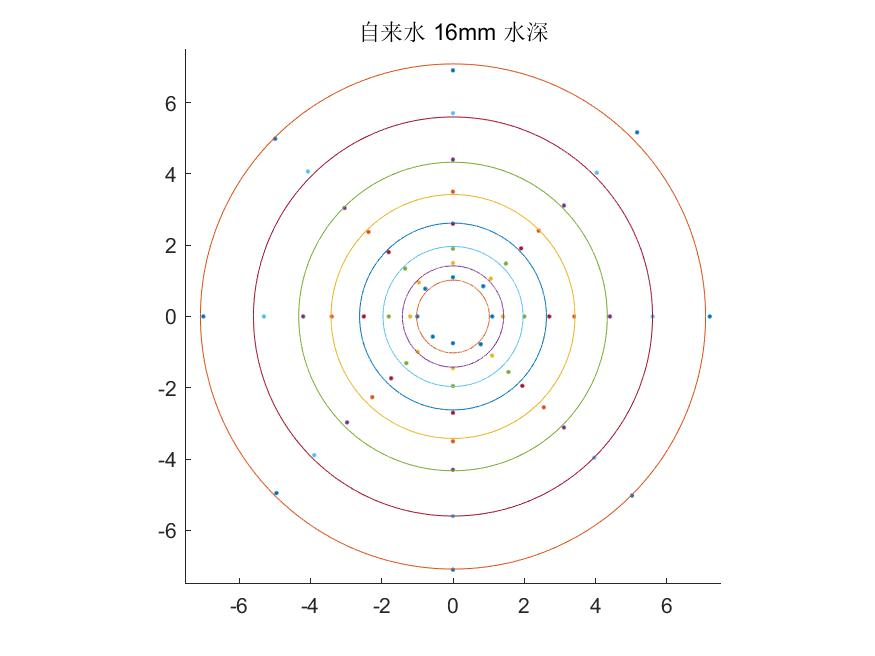
\includegraphics[width=.3\linewidth]{2.jpg}
            }
            \subfigure[]{
                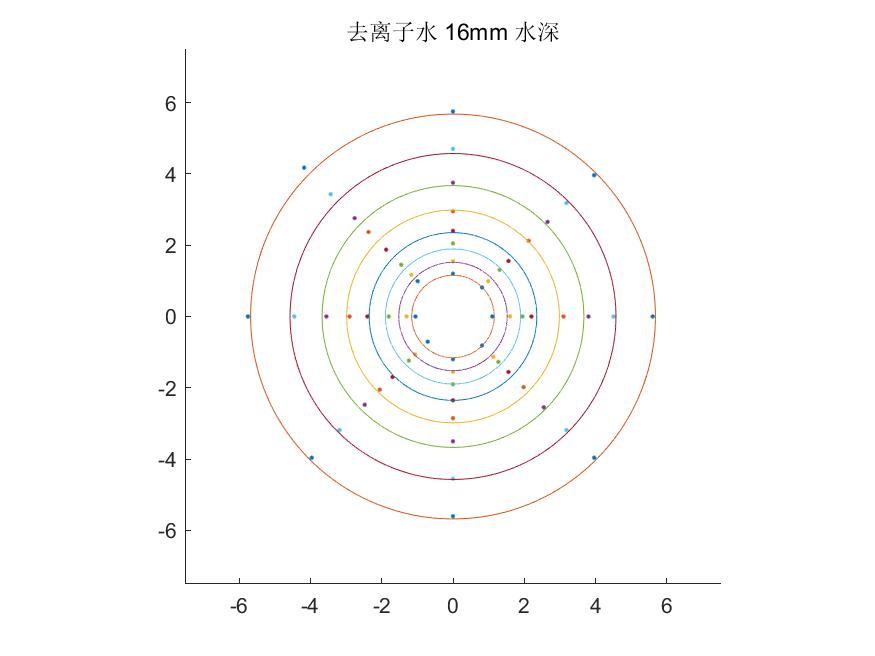
\includegraphics[width=.3\linewidth]{5.jpg}
            }
            \caption{16mm水深时自来水和去离子水的测绘结果}
            \begin{table}[]
                \begin{tabular}{|c|c|c|c|c|c|c|c|c|}
                \hline
                U/V  & 8    & 7    & 6    & 5    & 4    & 3    & 2    & 1    \\ \hline
                理论值  & 1.22 & 1.52 & 1.90 & 2.37 & 2.96 & 3.70 & 4.62 & 5.77 \\ \hline
                自来水  & 1.16 & 1.52 & 1.89 & 2.35 & 2.98 & 3.67 & 4.57 & 5.68 \\ \hline
                去离子水 & 1.02 & 1.42 & 1.96 & 2.62 & 3.42 & 4.33 & 5.59 & 7.08 \\ \hline
                \end{tabular}
            \end{table}
        
        \end{figure}
    
    \end{frame}

    \begin{frame}
        \frametitle{结果与分析}
        \textbf{结论}
        \begin{enumerate}
            \item 液体的深度对测绘结果有影响,但在液体的深度变化不大时(实验中为8mm~25mm),对测绘结果影响不大。
            \item 液体种类对测绘结果影响比较明显,使用自来水作为导电介质时较接近理论值,使用去离子水时偏差较大。
        \end{enumerate}
        
        \quad

        \textbf{误差来源}
        \begin{enumerate}
            \item 水的折射导致读数可能存在偏差。
            \item 使用电压表表笔测量电压时,难以保证表笔竖直。
            \item 测绘过程中水会被电解,可能会产生影响。
            \item 液体深度取值范围小,取值数量少,存在较在偶然误差。
            \item 实验装置精度不高,例如中心圆柱电极可能不在圆心,周围圆环电极可能不是个圆。
        \end{enumerate}
        
    
    \end{frame}

    \section{参考文献}

    \begin{frame}{参考文献}
        \begin{thebibliography}{99}  
            \bibitem{ref1}张兆奎, 缪连元, 张立, 钟菊花主编. 大学物理实验[M]. 北京, 高等教育出版社. 2016.8
            \bibitem{ref2}陈烨. 探测电路与导电介质对模拟静电场测绘的影响[J]. 杭州应用工程技术学院学报, 2000, 12(d):1-4
            \bibitem{ref3}郭慧敏. 全面分析静电场测绘实验误差[J]. 实验室科学, 2009(2):85-86
            \bibitem{ref4}傅金祝. 浅水交流电偶极矩水中电场的测量与分析[J]. 水雷战与战舰保护. 1997,10D: 6-9 
            \end{thebibliography}
    \end{frame}


\end{document}

  
   